\begin{figure}[h]
    \centering
    \begin{subfigure}[b]{0.9\textwidth}
        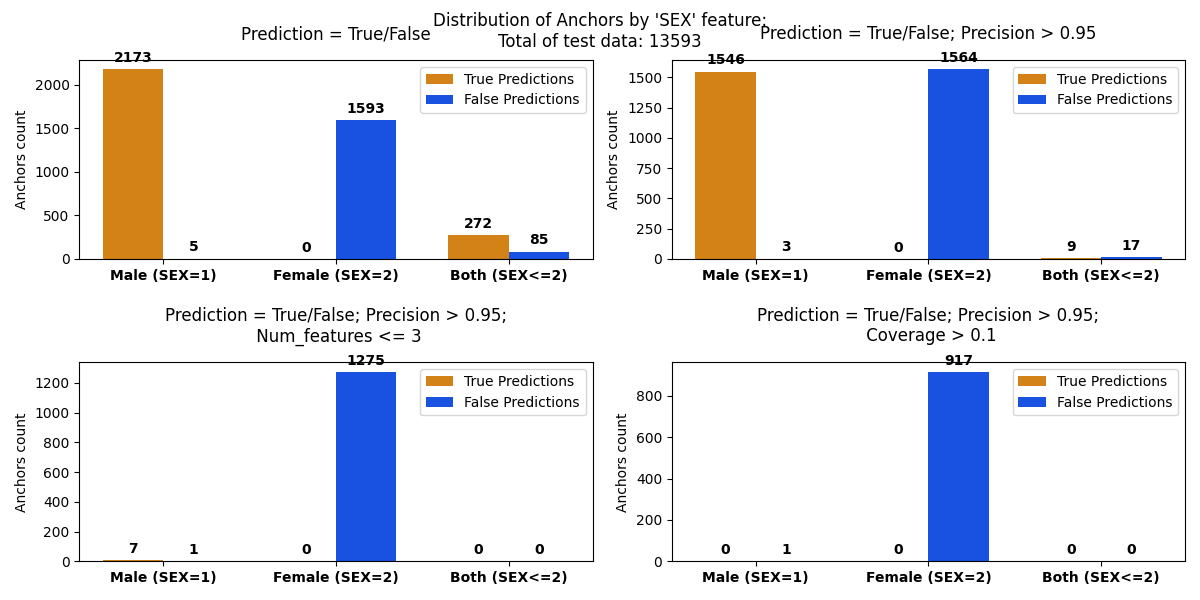
\includegraphics[width=\textwidth]{Images/distribution_folktables/pca_xg_tx_anchors.png}
        \caption{Model: XGBoost, XAI method: Anchors}
        \label{fig:distr_xg_tx_anchors}
    \end{subfigure}
    \hfill
    \begin{subfigure}[b]{0.9\textwidth}
        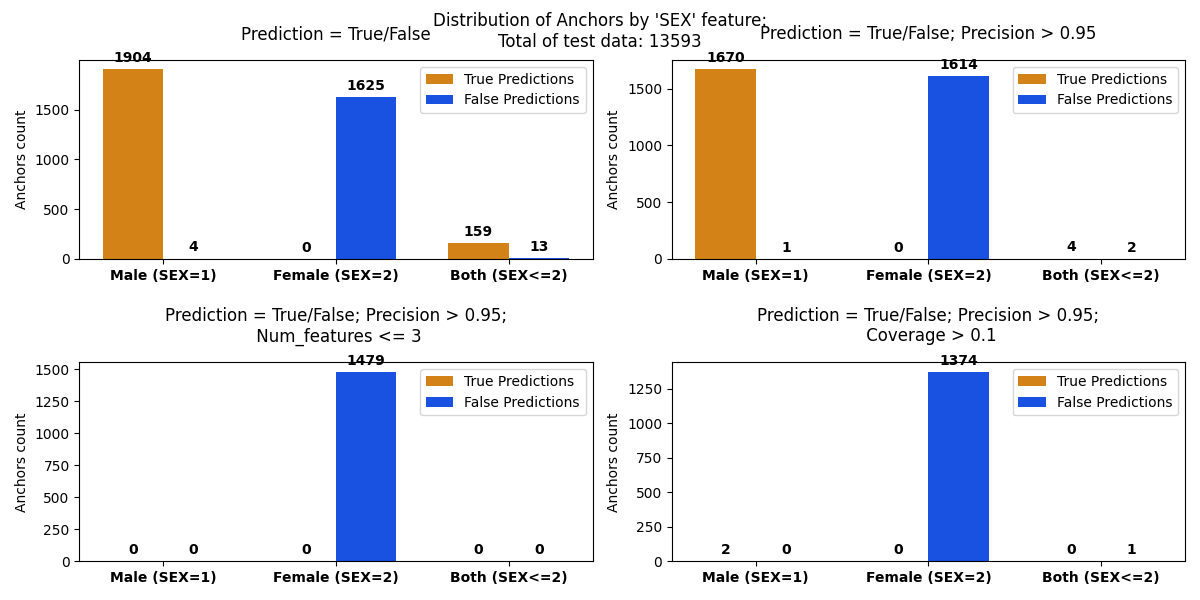
\includegraphics[width=\textwidth]{Images/distribution_folktables/pca_skrub_tx_anchors.png}
        \caption{Model: HistGradientBoosting, XAI method: Anchors}
        \label{fig:distr_skrub_tx_anchors}
    \end{subfigure}
    \caption{Comparison of the gendered explanations between True and False predictions in the Texas state (Part 1)}
 \end{figure}

\begin{figure}[h]
    \ContinuedFloat
    \begin{subfigure}[b]{0.9\textwidth}
        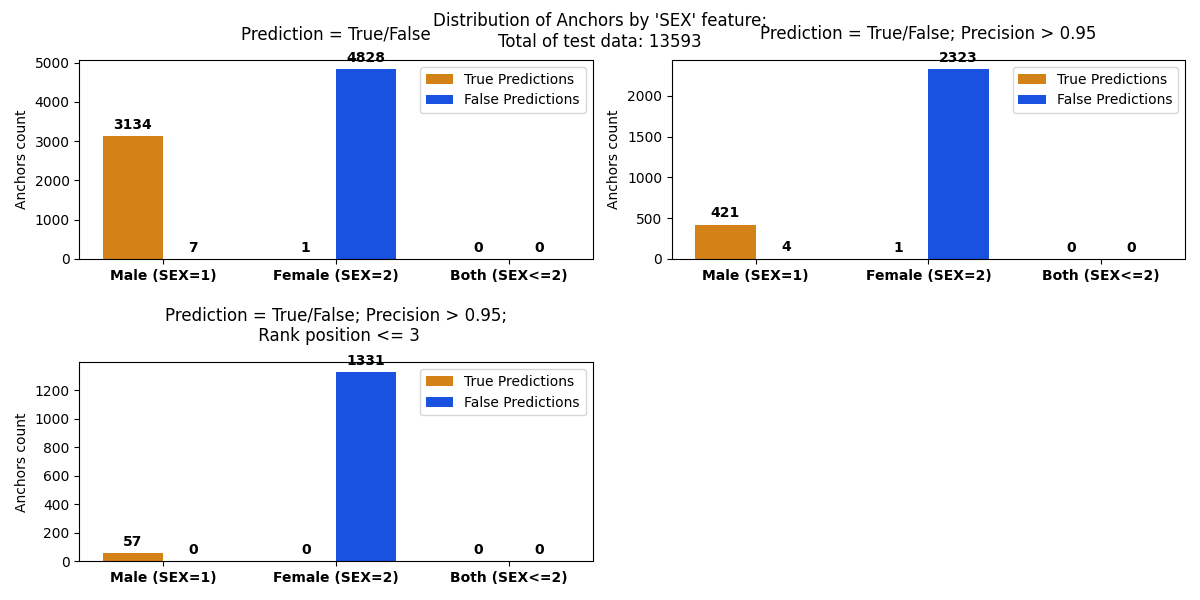
\includegraphics[width=\textwidth]{Images/distribution_folktables/pca_xg_tx_shap.png}
        \caption{Model: XGBoost, XAI method: SHAP}
        \label{fig:distr_xg_tx_shap}
    \end{subfigure}
    \hfill
    \begin{subfigure}[b]{0.9\textwidth}
        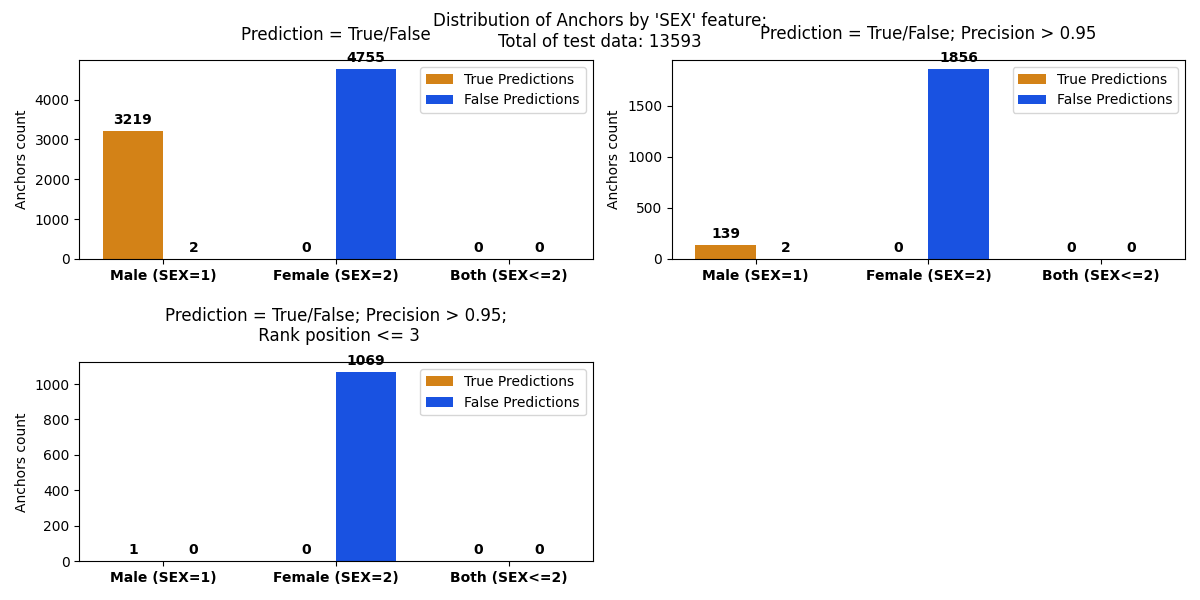
\includegraphics[width=\textwidth]{Images/distribution_folktables/pca_skrub_tx_shap.png}
        \caption{Model: HistGradientBoosting, XAI method: SHAP}
        \label{fig:distr_skrub_tx_shap}
    \end{subfigure}
    \caption{Comparison of the gendered explanations between True and False predictions in the Texas state (Part 2)}
    \label{fig:distr_tx}
\end{figure}
